I henhold til geometriske fremstillinger af lineære programmeringsproblemer er det nødvendigt at definere en række begreber.
Disse er \textit{hyperplan}, \textit{halvrum} og \textit{polyede}.
%
\begin{defn}{}{Polyede}
Lad $A$ være en $m \times n$ matrix, og lad $\mathbf{b}$ være en vektor i  $\R^m$.
En \textbf{polyede} er en mængde, der kan beskrives som 
$\{x\in \R^n \mid A\mathbf{x}\geq b\}.$
%
\end{defn}
\noindent
%
Som det fremgår fra definitionen, er en polyetop således mængden af mulige løsninger $\mathbf{x}$ af et ligningssystem.
Det gælder endvidere, at en mængde af formen $ \{x \in \R^n \mid A\textbf{x}=b,x \geq 0 \}$, hvilket kaldes en \textit{polyede på standardform}. 
% Kommentar til at der her er derfor det er rellevant og at det vil blive uddybet senere 
% Eventuelt med et eksempel 
%lidt forskellige muligheder her, enten kan det relateres til simplex eller blive introduceret her
%
Det gælder endvidere for polyeder at disse både kan være \textit{begrænsede} og \textit{ubegrænsede}.
%
\begin{defn}{}{}
En mængde $S \subset \R^n$ er \textbf{begrænset} såfremt der eksister en konstant $c$, hvorom det gælder, at den absolutte værdi af alle komponenter i alle elementer i $S$ er $\leq c$. 
Såfremt en sådan konstant ikke eksisterer er mængden \textbf{ubegrænset}. 
\end{defn}
\noindent
%
%alternativt værdien af ..... $\leq k$ eller $\geq$
%
I henhold til lineære programmeringsproblemer vil dette ofte være begrænset.
% Dette er eksempelvis tilfældet, hvis problemet er af en sådan karakter, at ingen af variabelene i karakterligningen kan have negative værdier.
%er det rigtigt det jeg skriver i ovenstående?
Ligeledes er det en fordel at definere polyeder, der er begrænset af kun én lineær betingelse. 
%
%skal der laves en definition på et polyede?
%
\begin{defn}{}{}
Lad $\mathbf{a}$ være en vektor i $\R^n$, hvor $\mathbf{a} \neq \mathbf{0}$ og lad $b$ være en skalar.
\begin{enumerate}[label=(\alph*)]
\item Mængden $\{x \in \R^n \mid \mathbf{a}^T \mathbf{x}=b\}$ kaldes et \textbf{hyperplan}.
\item Mængden $\{x \in \R^n \mid \mathbf{a}^T \mathbf{x} \geq b\}$ kaldes et \textbf{halvrum}.
\end{enumerate}
\end{defn}
\noindent
%
Det gælder her, at hyperplanet er grænsen for et tilsvarende halvrum.
I $\R^2$ vil hyperplanet således være en ret linje, som afskære en del af rummet, og der vil dermed være et halvrum på hver side af hyperplanet.
På figur \ref{fig:Graf123} ses et udsnit af hyperplanet, som afskærer et halvrum markeret med gråblå og et halvrum markeret med orangerød. 

%%%%%%%%%%%%%%%%%%%%%%%%%%%%%%%%
%%% Flot graf alla Julie     %%%
%%%%%%%%%%%%%%%%%%%%%%%%%%%%%%%%
\begin{center}
\begin{tikzpicture}
% Den øverste linje
\draw[name path=b,-, white, thick] (0,3.5) -- (6,3.5);
%
% Den nederste linje
\draw[name path=c,-, white, thick] (0,-1) -- (6,-1);
%
% Den mellemste linje
\draw[name path=a,-, white, thick] (0,0) -- (6,3);
%
% Farvning 
\tikzfillbetween [of=a and b]{myblue!5}
\tikzfillbetween [of=a and c]{myred!5}
%
% Linjen mellem 
\draw[-, black, very thick] (0,0) -- (6,3);
\draw[->, black, thick] (2.4,1.2) -- (2,2);
\filldraw[black] (0.2,-0.3) circle (0pt) node[anchor=west] {$\mathbf{a}^T \mathbf{x}=b$};
\filldraw[black] (3,2.6) circle (0pt) node[anchor=west] {$\mathbf{a}^T \mathbf{x} > b$};
\filldraw[black] (3,1.3) circle (0pt) node[anchor=west] {$\mathbf{a}^T \mathbf{x} < b$};
\filldraw[black] (1.6,2.2) circle (0pt) node[anchor=west] {$\mathbf{a}$};
\end{tikzpicture}
  \captionof{figure}{Et hyperplan og to halvrum, markeret med henholdsvis gråblå for $\mathbf{a}^T \mathbf{x} < b$ og orangerød for $\mathbf{a}^T \mathbf{x} > b$.}
  \label{fig:Graf123}
\end{center}
%
%\begin{center}
%\begin{tikzpicture}
%\begin{axis}
%\addplot3[
%    surf,
%]
%{0.5*x};
%\end{axis}
%\end{tikzpicture}
%  \captionof{figure}{FUCK DET HER LORT XD}
%  \label{fig:NEJ}
%\end{center}
% 
%%%%%%%%%%%%%%%%%%%%%%%%%%%%%%%%
%%% Flot graf alla Julie     %%%
%%%%%%%%%%%%%%%%%%%%%%%%%%%%%%%%
%
\begin{center}
%start tikz picture, and use the tdplot_main_coords style to implement the display 
%coordinate transformation provided by 3dplot
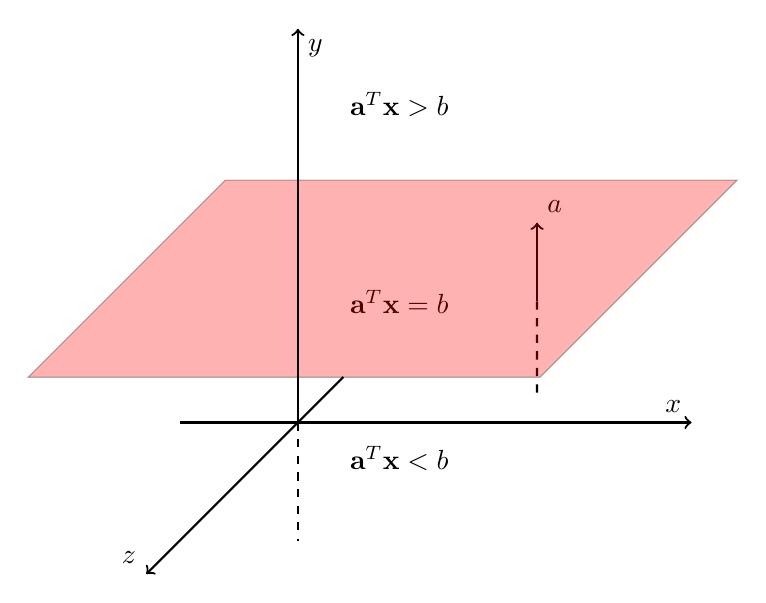
\begin{tikzpicture}[scale=5]%[scale=5,tdplot_main_coords]
%set up some coordinates 
%-----------------------
\coordinate (O) at (0,0,0);
\coordinate (XZ) at (1,0,1);
\coordinate (X) at (1,0,-0.3);
\coordinate (Z) at (-0.3,0,1);
\coordinate (Y) at (-0.3,0,-0.3);
%
\coordinate (XZa) at (1,0.5,1);
\coordinate (Xa) at (1,0.5,-0.3);
\coordinate (Za) at (-0.3,0.5,1);
\coordinate (Ya) at (-0.3,0.5,-0.3);
%
\coordinate (Na) at (0.8,0.5,0.5);
\coordinate (Pa) at (0.8,0.7,0.5);
%
\coordinate (N) at (0.5,0,0.5);
\coordinate (P) at (0.5,0.5,0.5);
%
\draw[black] (0.3,0.5,0.5) circle (0pt) node[anchor=west] {$\mathbf{a}^T \mathbf{x}=b$};
\draw[black] (0.3,1,0.5) circle (0pt) node[anchor=west] {$\mathbf{a}^T \mathbf{x} > b$};
\draw[black] (0.3,0.1,0.5) circle (0pt) node[anchor=west] {$\mathbf{a}^T \mathbf{x} < b$};
%
%draw figure contents
%--------------------
\draw [thick,->] (Na) -- (Pa) node[anchor=south west]{$a$};
\draw [thick, dashed] (Na) -- (0.8,0.25,0.5);
%
\filldraw [fill=red,opacity=0.3] 
         (Ya) -- (Xa) -- (XZa) -- (Za) -- cycle;
%
%draw the main coordinate system axes
\draw[thick,->] (0,0,0) -- (1,0,0) node[anchor=south east]{$x$};
\draw[thick] (0,0,0) -- (-0.3,0,0);
\draw[thick,->] (0,0,0) -- (0,1,0) node[anchor=north west]{$y$};
\draw[thick,dashed] (0,0,0) -- (0,-0.3,0);
\draw[thick,->] (0,0,0) -- (0,0,1) node[anchor=south east]{$z$};
\draw[thick] (0,0,0) -- (0,0,-0.3);
\end{tikzpicture}
  \captionof{figure}{Et hyperplan i $\R^3$ og to halvrum.}
  \label{fig:mm}
\end{center}
%
%Et polyhedron er derfor en samling af polyeder der til sammen skaber en geometrisk figur i et givet vektorrum.
%
\begin{thm}{}{}
Lad $\mathbf{a}$ være en vektor i $\R^n$, hvor 
$\mathbf{a} \neq \mathbf{0}.$
For hyperplanet 
$\{x \in \R^n \mid \mathbf{a}^T \mathbf{x}=b\},$ 
vil $\mathbf{a}$ være ortogonal med hyperplanet.
\end{thm}
% 
\begin{proof}
Lad $\mathbf{x}$ og $\mathbf{y}$ tilhører det samme hyperplan, så er $\mathbf{a}^Tx=\mathbf{a}^Ty.$
Dermed er $\mathbf{a}^T(x-y)=0$, og så er $\mathbf{a}$ ortogonal til alle vektorer i hyperplanet. 
\end{proof}